\documentclass[12pt,a4paper]{article}
\usepackage[utf8]{inputenc}
\usepackage[english]{babel}
\usepackage{appendix}
\usepackage{listings}
\usepackage{xcolor}
\usepackage{graphicx}
\graphicspath{ {./} }

\definecolor{backcolour}{rgb}{0.9,0.9,0.9}

\lstdefinestyle{lstyle}{
    backgroundcolor=\color{backcolour},                 
    numbers=left,                    
    numbersep=5pt,                  
}

\lstset{style=lstyle}

\author{Andrei N. Onea}
\title{37212-cwk1-S-Segmentation\_k83954ao}

\begin{document}
\maketitle

\section*{Experiments}

This assignment proposes a look at performing thresholding on an image in order to find edges. The process the image goes through is filtering, followed by the application of the Sobel kernels to compute the image gradients in the X-axis and Y-axis, which are then combined to get the image gradient magnitude. Finally, by producing a histogram, we find a feasible threshold value to segment the image by. We will compare two filtering methods, using a mean filter for the smoothing and a weighted-mean filter. The subject of this experiment is this cute kitten here in figure \ref{fig:kitty}.

\begin{figure}[h]
    \centering
    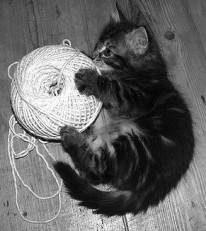
\includegraphics[width=0.5\textwidth]{kitty}
    \caption{A nice kitty}
    \label{fig:kitty}
\end{figure}

\newpage

\section*{Preparation}

For the purpose of this assignment, Python has been chosen as the implementation language and most of the functions have been written from scratch. In fact, the only image processing function used that has not been written from scratch is the one that calculates the image histogram. Numpy arrays have been used for the processing of the matrices and OpenCV for I/O image functions. The convolution function iterates through each pixel in the input image and multiplies it with the corresponding value in the moving window of the kernel. The input image is padded before the operation to deal with the edges and corners, and then normalized in binary64 precision for accuracy. The two filtering kernels are described in the next sections.

\subsubsection*{Mean filter}

The mean filter is a very simple smoothing kernel which replaces each pixel value with the average of itself and all its neighbours. The disadvantage is that this method does not take into account the spatiality of the pixels, meaning that a neighbouring pixel, which does not represent the same object the current pixel does, will still have an equal amount of influence on the resulting pixel.

\subsubsection*{Weighted-mean filter}

The weighted-mean filter accounts for the issue mentioned previously by setting a weight for each element in the kernel. To choose the values, a two-dimensional Gaussian distribution function has been implemented, the output of which is the classic bell-shaped curve. Thus, a normal distribution of the numbers is created which are then normalized prior to the convolution.

\section*{Results}

\subsubsection*{Smoothing}

Both kernels are 7x7 in size. For the weighted-mean kernel, an amplitude of 5 and a spread of $0.25$ on both axes has been chosen, but the size makes the most difference. These parameters produce the bell curve in figure \ref{fig:bell} and extremely similar outputs, as seen in figures \ref{fig:msobel} and \ref{fig:gsobel}.

\begin{figure}[ht]
    \centering
    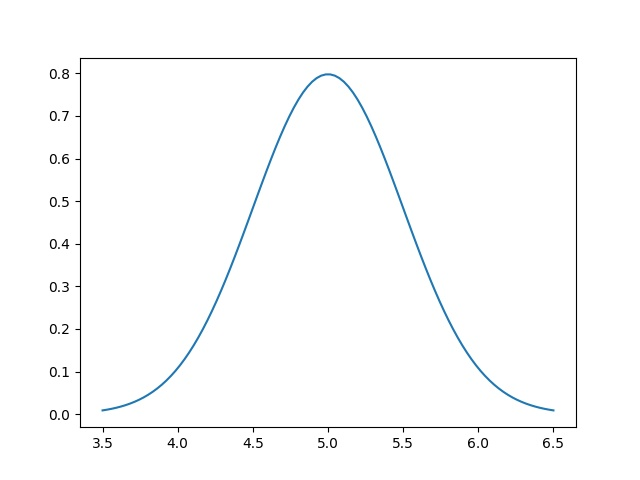
\includegraphics[width=0.75\textwidth]{bell}
    \caption{Gaussian distribution for the weighted-mean kernel}
    \label{fig:bell}
\end{figure}

\subsubsection*{Sobel kernel}

The Sobel kernels detect edges separately in both axes. The filtered images from the previous steps are convolved using Sobel and the resulting image gradients are combined to form the image magnitude. Output present in figures \ref{fig:msobel} and \ref{fig:gsobel}.

\begin{figure}[ht]
    \centering
    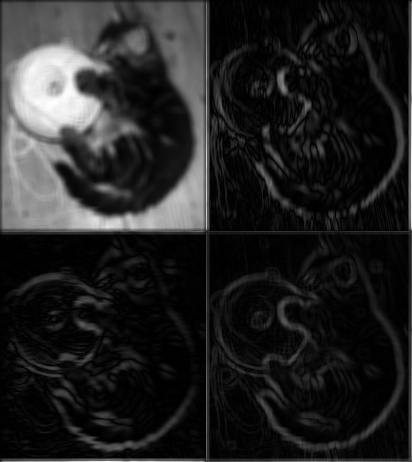
\includegraphics[width=0.5\textwidth]{msobel}
    \caption{Image smoothed using a 7x7 mean kernel; top-left: smoothed image, top-right: X gradient, bottom-left: Y gradient, bottom-right: image magnitude}
    \label{fig:msobel}
\end{figure}

\begin{figure}[ht]
    \centering
    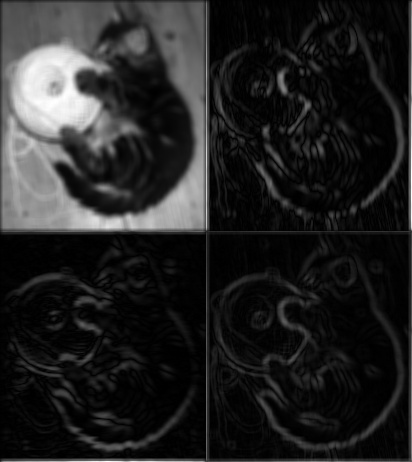
\includegraphics[width=0.5\textwidth]{gsobel}
    \caption{Image smoothed using a 7x7 weighted-mean kernel with amplitude 5 and spread 0.25; top-left: smoothed image, top-right: X gradient, bottom-left: Y gradient, bottom-right: image magnitude}
    \label{fig:gsobel}
\end{figure}

\subsubsection*{Thresholding}

The edge strength images are then passed through a threshold function. The value for this function was chosen by looking at the histogram of the magnitude image and picking the value where the rate of change becomes smaller than near the peak. Histograms visible in  figure \ref{fig:hist} and results in figure \ref{fig:edge}.

\begin{figure}[ht]
    \centering
    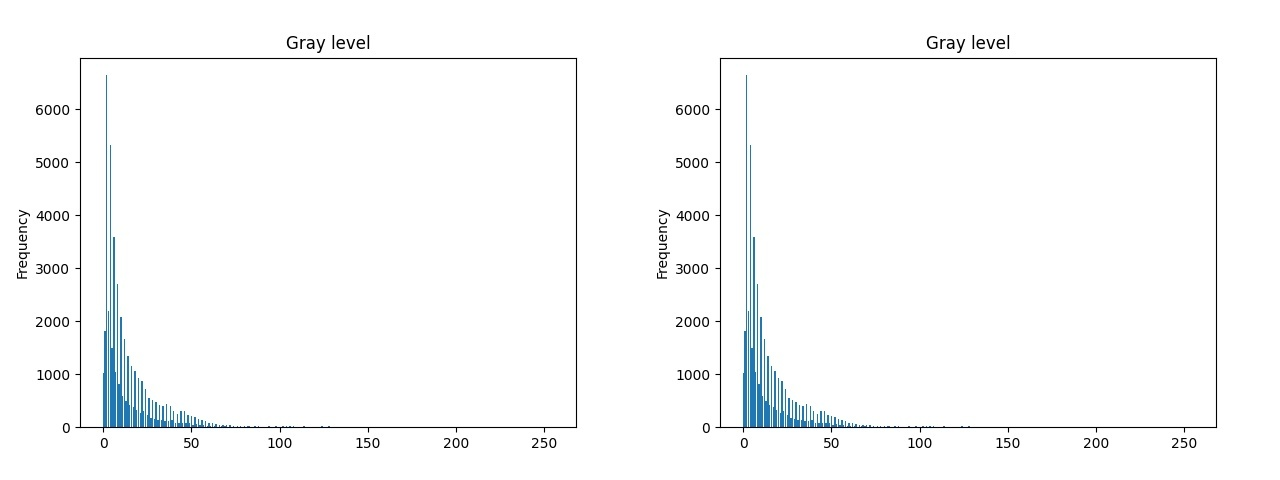
\includegraphics[width=1\textwidth]{hist}
    \caption{Histograms; left: mean kernel, right: weighted-mean kernel}
    \label{fig:hist}
\end{figure}

\begin{figure}[ht]
    \centering
    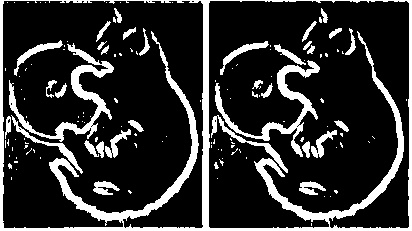
\includegraphics[width=0.75\textwidth]{edge}
    \caption{Edges found; left: mean kernel, right: weighted-mean kernel}
    \label{fig:edge}
\end{figure}

\section*{Conclusion}

Figure \ref{fig:diff} shows the difference between the two edge images. I have tried many tweaks for the Gaussian distribution, but I could not find a set of values that separates the two results by a greater margin.

\begin{figure}[ht]
    \centering
    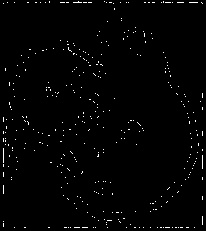
\includegraphics[width=0.5\textwidth]{img_edge_comparison}
    \caption{Difference image between the two results; left: mean kernel, right: weighted-mean kernel}
    \label{fig:diff}
\end{figure}

\end{document}